% Created by tikzDevice version 0.12.3.1 on 2021-06-04 21:11:52
% !TEX encoding = UTF-8 Unicode
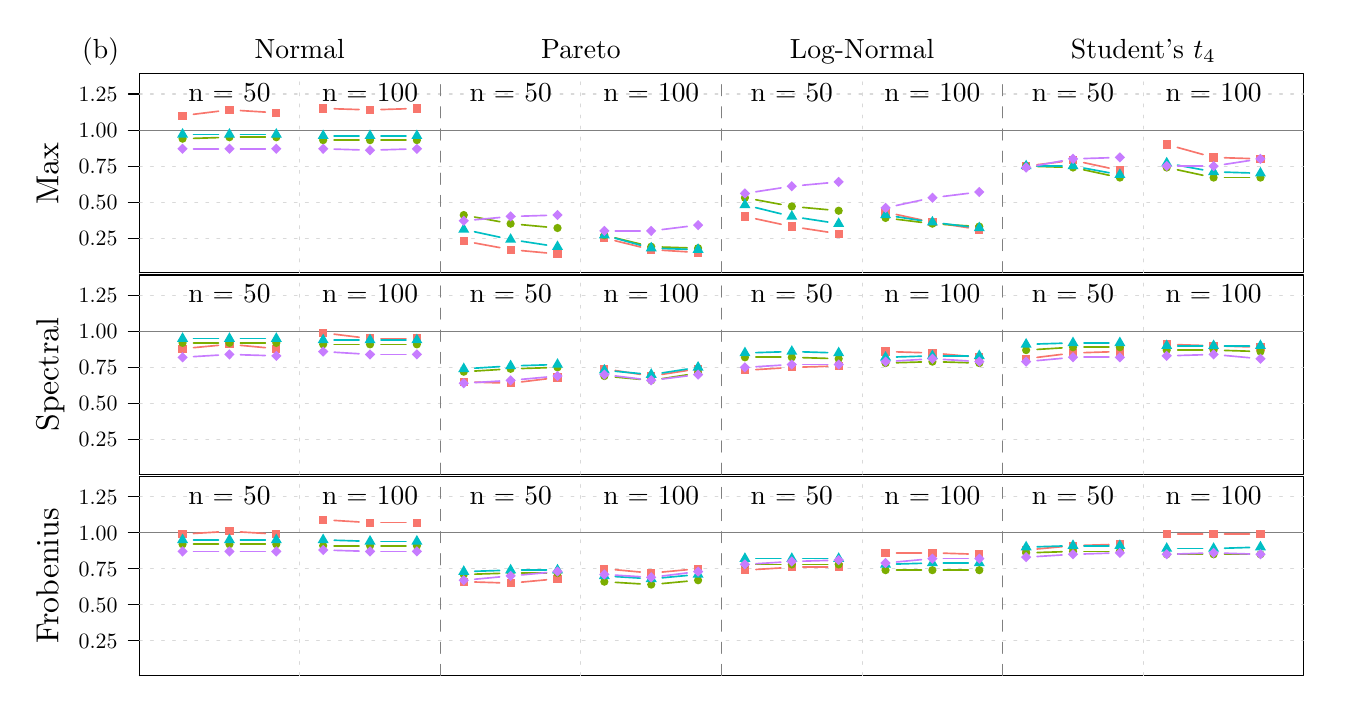
\begin{tikzpicture}[x=1pt,y=1pt]
\definecolor{fillColor}{RGB}{255,255,255}
\path[use as bounding box,fill=fillColor,fill opacity=0.00] (0,0) rectangle (469.76,234.88);
\begin{scope}
\path[clip] (  0.00,  0.00) rectangle (469.76,234.88);
\definecolor{drawColor}{RGB}{0,0,0}

\path[draw=drawColor,line width= 0.4pt,line join=round,line cap=round] ( 40.39,146.29) --
	(461.04,146.29) --
	(461.04,218.25) --
	( 40.39,218.25) --
	( 40.39,146.29);

\path[draw=drawColor,line width= 0.4pt,line join=round,line cap=round] ( 40.39,158.84) -- ( 40.39,210.90);

\path[draw=drawColor,line width= 0.4pt,line join=round,line cap=round] ( 40.39,158.84) -- ( 36.43,158.84);

\path[draw=drawColor,line width= 0.4pt,line join=round,line cap=round] ( 40.39,171.86) -- ( 36.43,171.86);

\path[draw=drawColor,line width= 0.4pt,line join=round,line cap=round] ( 40.39,184.87) -- ( 36.43,184.87);

\path[draw=drawColor,line width= 0.4pt,line join=round,line cap=round] ( 40.39,197.88) -- ( 36.43,197.88);

\path[draw=drawColor,line width= 0.4pt,line join=round,line cap=round] ( 40.39,210.90) -- ( 36.43,210.90);

\node[text=drawColor,anchor=base east,inner sep=0pt, outer sep=0pt, scale=  0.79] at ( 32.47,156.12) {0.25};

\node[text=drawColor,anchor=base east,inner sep=0pt, outer sep=0pt, scale=  0.79] at ( 32.47,169.13) {0.50};

\node[text=drawColor,anchor=base east,inner sep=0pt, outer sep=0pt, scale=  0.79] at ( 32.47,182.14) {0.75};

\node[text=drawColor,anchor=base east,inner sep=0pt, outer sep=0pt, scale=  0.79] at ( 32.47,195.16) {1.00};

\node[text=drawColor,anchor=base east,inner sep=0pt, outer sep=0pt, scale=  0.79] at ( 32.47,208.17) {1.25};
\end{scope}
\begin{scope}
\path[clip] ( 40.39,146.29) rectangle (461.04,218.25);
\definecolor{drawColor}{gray}{0.85}

\path[draw=drawColor,line width= 0.4pt,dash pattern=on 1pt off 3pt ,line join=round,line cap=round] ( 40.39,158.84) -- (461.04,158.84);

\path[draw=drawColor,line width= 0.4pt,dash pattern=on 1pt off 3pt ,line join=round,line cap=round] ( 40.39,171.86) -- (461.04,171.86);

\path[draw=drawColor,line width= 0.4pt,dash pattern=on 1pt off 3pt ,line join=round,line cap=round] ( 40.39,184.87) -- (461.04,184.87);

\path[draw=drawColor,line width= 0.4pt,dash pattern=on 1pt off 3pt ,line join=round,line cap=round] ( 40.39,197.88) -- (461.04,197.88);

\path[draw=drawColor,line width= 0.4pt,dash pattern=on 1pt off 3pt ,line join=round,line cap=round] ( 40.39,210.90) -- (461.04,210.90);

\path[draw=drawColor,line width= 0.4pt,dash pattern=on 1pt off 3pt ,line join=round,line cap=round] ( 98.31,146.29) -- ( 98.31,218.25);

\path[draw=drawColor,line width= 0.4pt,dash pattern=on 1pt off 3pt ,line join=round,line cap=round] (199.91,146.29) -- (199.91,218.25);

\path[draw=drawColor,line width= 0.4pt,dash pattern=on 1pt off 3pt ,line join=round,line cap=round] (301.52,146.29) -- (301.52,218.25);

\path[draw=drawColor,line width= 0.4pt,dash pattern=on 1pt off 3pt ,line join=round,line cap=round] (403.13,146.29) -- (403.13,218.25);
\definecolor{drawColor}{gray}{0.50}

\path[draw=drawColor,line width= 0.4pt,dash pattern=on 4pt off 4pt ,line join=round,line cap=round] (149.11,146.29) -- (149.11,218.25);

\path[draw=drawColor,line width= 0.4pt,dash pattern=on 4pt off 4pt ,line join=round,line cap=round] (250.72,146.29) -- (250.72,218.25);

\path[draw=drawColor,line width= 0.4pt,dash pattern=on 4pt off 4pt ,line join=round,line cap=round] (352.32,146.29) -- (352.32,218.25);
\end{scope}
\begin{scope}
\path[clip] (  0.00,  0.00) rectangle (469.76,234.88);
\definecolor{drawColor}{RGB}{0,0,0}

\node[text=drawColor,rotate= 90.00,anchor=base,inner sep=0pt, outer sep=0pt, scale=  1.15] at ( 11.09,182.27) {Max};
\end{scope}
\begin{scope}
\path[clip] ( 40.39,146.29) rectangle (461.04,218.25);
\definecolor{drawColor}{gray}{0.50}

\path[draw=drawColor,line width= 0.4pt,line join=round,line cap=round] ( 40.39,197.88) -- (461.04,197.88);
\end{scope}
\begin{scope}
\path[clip] (  0.00,  0.00) rectangle (469.76,234.88);
\definecolor{drawColor}{RGB}{0,0,0}

\node[text=drawColor,anchor=base,inner sep=0pt, outer sep=0pt, scale=  1.00] at ( 26.34,223.79) {(b)};

\node[text=drawColor,anchor=base,inner sep=0pt, outer sep=0pt, scale=  1.00] at ( 98.31,223.79) {Normal};

\node[text=drawColor,anchor=base,inner sep=0pt, outer sep=0pt, scale=  1.00] at (199.91,223.79) {Pareto};

\node[text=drawColor,anchor=base,inner sep=0pt, outer sep=0pt, scale=  1.00] at (301.52,223.79) {Log-Normal};

\node[text=drawColor,anchor=base,inner sep=0pt, outer sep=0pt, scale=  1.00] at (403.13,223.79) {Student's $t_4$};
\end{scope}
\begin{scope}
\path[clip] ( 40.39,146.29) rectangle (461.04,218.25);
\definecolor{drawColor}{RGB}{0,0,0}

\node[text=drawColor,anchor=base,inner sep=0pt, outer sep=0pt, scale=  0.99] at ( 72.91,208.20) {n = 50};

\node[text=drawColor,anchor=base,inner sep=0pt, outer sep=0pt, scale=  0.99] at (123.71,208.20) {n = 100};

\node[text=drawColor,anchor=base,inner sep=0pt, outer sep=0pt, scale=  0.99] at (174.51,208.20) {n = 50};

\node[text=drawColor,anchor=base,inner sep=0pt, outer sep=0pt, scale=  0.99] at (225.32,208.20) {n = 100};

\node[text=drawColor,anchor=base,inner sep=0pt, outer sep=0pt, scale=  0.99] at (276.12,208.20) {n = 50};

\node[text=drawColor,anchor=base,inner sep=0pt, outer sep=0pt, scale=  0.99] at (326.92,208.20) {n = 100};

\node[text=drawColor,anchor=base,inner sep=0pt, outer sep=0pt, scale=  0.99] at (377.73,208.20) {n = 50};

\node[text=drawColor,anchor=base,inner sep=0pt, outer sep=0pt, scale=  0.99] at (428.53,208.20) {n = 100};
\definecolor{drawColor}{RGB}{248,118,109}

\path[draw=drawColor,line width= 0.6pt,line join=round,line cap=round] ( 59.90,203.57) -- ( 68.98,204.69);

\path[draw=drawColor,line width= 0.6pt,line join=round,line cap=round] ( 76.86,204.93) -- ( 85.89,204.37);
\definecolor{fillColor}{RGB}{248,118,109}

\path[fill=fillColor] ( 54.49,201.60) --
	( 57.46,201.60) --
	( 57.46,204.57) --
	( 54.49,204.57) --
	cycle;

\path[fill=fillColor] ( 71.42,203.69) --
	( 74.39,203.69) --
	( 74.39,206.66) --
	( 71.42,206.66) --
	cycle;

\path[fill=fillColor] ( 88.36,202.64) --
	( 91.33,202.64) --
	( 91.33,205.61) --
	( 88.36,205.61) --
	cycle;
\definecolor{drawColor}{RGB}{124,174,0}

\path[draw=drawColor,line width= 0.6pt,line join=round,line cap=round] ( 59.93,194.88) -- ( 68.95,195.16);

\path[draw=drawColor,line width= 0.6pt,line join=round,line cap=round] ( 76.87,195.28) -- ( 85.88,195.28);
\definecolor{fillColor}{RGB}{124,174,0}

\path[fill=fillColor] ( 55.97,194.76) circle (  1.49);

\path[fill=fillColor] ( 72.91,195.28) circle (  1.49);

\path[fill=fillColor] ( 89.84,195.28) circle (  1.49);
\definecolor{drawColor}{RGB}{0,191,196}

\path[draw=drawColor,line width= 0.6pt,line join=round,line cap=round] ( 59.93,196.32) -- ( 68.95,196.32);

\path[draw=drawColor,line width= 0.6pt,line join=round,line cap=round] ( 76.87,196.32) -- ( 85.88,196.32);
\definecolor{fillColor}{RGB}{0,191,196}

\path[fill=fillColor] ( 55.97,198.63) --
	( 57.97,195.17) --
	( 53.97,195.17) --
	cycle;

\path[fill=fillColor] ( 72.91,198.63) --
	( 74.91,195.17) --
	( 70.91,195.17) --
	cycle;

\path[fill=fillColor] ( 89.84,198.63) --
	( 91.84,195.17) --
	( 87.84,195.17) --
	cycle;
\definecolor{drawColor}{RGB}{199,124,255}

\path[draw=drawColor,line width= 0.6pt,line join=round,line cap=round] ( 59.93,191.12) -- ( 68.95,191.12);

\path[draw=drawColor,line width= 0.6pt,line join=round,line cap=round] ( 76.87,191.12) -- ( 85.88,191.12);
\definecolor{fillColor}{RGB}{199,124,255}

\path[fill=fillColor] ( 54.12,191.12) --
	( 55.97,192.97) --
	( 57.83,191.12) --
	( 55.97,189.26) --
	cycle;

\path[fill=fillColor] ( 71.05,191.12) --
	( 72.91,192.97) --
	( 74.76,191.12) --
	( 72.91,189.26) --
	cycle;

\path[fill=fillColor] ( 87.98,191.12) --
	( 89.84,192.97) --
	( 91.70,191.12) --
	( 89.84,189.26) --
	cycle;
\definecolor{drawColor}{RGB}{248,118,109}

\path[draw=drawColor,line width= 0.6pt,line join=round,line cap=round] (110.73,205.57) -- (119.75,205.29);

\path[draw=drawColor,line width= 0.6pt,line join=round,line cap=round] (127.67,205.29) -- (136.69,205.57);
\definecolor{fillColor}{RGB}{248,118,109}

\path[fill=fillColor] (105.29,204.21) --
	(108.26,204.21) --
	(108.26,207.18) --
	(105.29,207.18) --
	cycle;

\path[fill=fillColor] (122.22,203.69) --
	(125.19,203.69) --
	(125.19,206.66) --
	(122.22,206.66) --
	cycle;

\path[fill=fillColor] (139.16,204.21) --
	(142.13,204.21) --
	(142.13,207.18) --
	(139.16,207.18) --
	cycle;
\definecolor{drawColor}{RGB}{124,174,0}

\path[draw=drawColor,line width= 0.6pt,line join=round,line cap=round] (110.73,194.24) -- (119.75,194.24);

\path[draw=drawColor,line width= 0.6pt,line join=round,line cap=round] (127.67,194.24) -- (136.68,194.24);
\definecolor{fillColor}{RGB}{124,174,0}

\path[fill=fillColor] (106.77,194.24) circle (  1.49);

\path[fill=fillColor] (123.71,194.24) circle (  1.49);

\path[fill=fillColor] (140.64,194.24) circle (  1.49);
\definecolor{drawColor}{RGB}{0,191,196}

\path[draw=drawColor,line width= 0.6pt,line join=round,line cap=round] (110.73,195.80) -- (119.75,195.80);

\path[draw=drawColor,line width= 0.6pt,line join=round,line cap=round] (127.67,195.80) -- (136.68,195.80);
\definecolor{fillColor}{RGB}{0,191,196}

\path[fill=fillColor] (106.77,198.11) --
	(108.77,194.65) --
	(104.77,194.65) --
	cycle;

\path[fill=fillColor] (123.71,198.11) --
	(125.71,194.65) --
	(121.71,194.65) --
	cycle;

\path[fill=fillColor] (140.64,198.11) --
	(142.64,194.65) --
	(138.64,194.65) --
	cycle;
\definecolor{drawColor}{RGB}{199,124,255}

\path[draw=drawColor,line width= 0.6pt,line join=round,line cap=round] (110.73,190.99) -- (119.75,190.72);

\path[draw=drawColor,line width= 0.6pt,line join=round,line cap=round] (127.67,190.72) -- (136.69,190.99);
\definecolor{fillColor}{RGB}{199,124,255}

\path[fill=fillColor] (104.92,191.12) --
	(106.77,192.97) --
	(108.63,191.12) --
	(106.77,189.26) --
	cycle;

\path[fill=fillColor] (121.85,190.60) --
	(123.71,192.45) --
	(125.57,190.60) --
	(123.71,188.74) --
	cycle;

\path[fill=fillColor] (138.79,191.12) --
	(140.64,192.97) --
	(142.50,191.12) --
	(140.64,189.26) --
	cycle;
\definecolor{drawColor}{RGB}{248,118,109}

\path[draw=drawColor,line width= 0.6pt,line join=round,line cap=round] (161.47,157.08) -- (170.62,155.40);

\path[draw=drawColor,line width= 0.6pt,line join=round,line cap=round] (178.46,154.32) -- (187.50,153.48);
\definecolor{fillColor}{RGB}{248,118,109}

\path[fill=fillColor] (156.09,156.32) --
	(159.06,156.32) --
	(159.06,159.29) --
	(156.09,159.29) --
	cycle;

\path[fill=fillColor] (173.03,153.19) --
	(176.00,153.19) --
	(176.00,156.16) --
	(173.03,156.16) --
	cycle;

\path[fill=fillColor] (189.96,151.63) --
	(192.93,151.63) --
	(192.93,154.60) --
	(189.96,154.60) --
	cycle;
\definecolor{drawColor}{RGB}{124,174,0}

\path[draw=drawColor,line width= 0.6pt,line join=round,line cap=round] (161.47,166.45) -- (170.62,164.77);

\path[draw=drawColor,line width= 0.6pt,line join=round,line cap=round] (178.46,163.69) -- (187.50,162.85);
\definecolor{fillColor}{RGB}{124,174,0}

\path[fill=fillColor] (157.58,167.17) circle (  1.49);

\path[fill=fillColor] (174.51,164.05) circle (  1.49);

\path[fill=fillColor] (191.45,162.49) circle (  1.49);
\definecolor{drawColor}{RGB}{0,191,196}

\path[draw=drawColor,line width= 0.6pt,line join=round,line cap=round] (161.45,161.13) -- (170.64,159.16);

\path[draw=drawColor,line width= 0.6pt,line join=round,line cap=round] (178.43,157.72) -- (187.53,156.32);
\definecolor{fillColor}{RGB}{0,191,196}

\path[fill=fillColor] (157.58,164.28) --
	(159.58,160.81) --
	(155.58,160.81) --
	cycle;

\path[fill=fillColor] (174.51,160.63) --
	(176.51,157.17) --
	(172.51,157.17) --
	cycle;

\path[fill=fillColor] (191.45,158.03) --
	(193.45,154.57) --
	(189.45,154.57) --
	cycle;
\definecolor{drawColor}{RGB}{199,124,255}

\path[draw=drawColor,line width= 0.6pt,line join=round,line cap=round] (161.52,165.45) -- (170.57,166.29);

\path[draw=drawColor,line width= 0.6pt,line join=round,line cap=round] (178.47,166.77) -- (187.49,167.05);
\definecolor{fillColor}{RGB}{199,124,255}

\path[fill=fillColor] (155.72,165.09) --
	(157.58,166.95) --
	(159.43,165.09) --
	(157.58,163.23) --
	cycle;

\path[fill=fillColor] (172.66,166.65) --
	(174.51,168.51) --
	(176.37,166.65) --
	(174.51,164.80) --
	cycle;

\path[fill=fillColor] (189.59,167.17) --
	(191.45,169.03) --
	(193.30,167.17) --
	(191.45,165.32) --
	cycle;
\definecolor{drawColor}{RGB}{248,118,109}

\path[draw=drawColor,line width= 0.6pt,line join=round,line cap=round] (212.23,157.90) -- (221.47,155.63);

\path[draw=drawColor,line width= 0.6pt,line join=round,line cap=round] (229.27,154.44) -- (238.30,153.88);
\definecolor{fillColor}{RGB}{248,118,109}

\path[fill=fillColor] (206.90,157.36) --
	(209.87,157.36) --
	(209.87,160.33) --
	(206.90,160.33) --
	cycle;

\path[fill=fillColor] (223.83,153.19) --
	(226.80,153.19) --
	(226.80,156.16) --
	(223.83,156.16) --
	cycle;

\path[fill=fillColor] (240.77,152.15) --
	(243.74,152.15) --
	(243.74,155.12) --
	(240.77,155.12) --
	cycle;
\definecolor{drawColor}{RGB}{124,174,0}

\path[draw=drawColor,line width= 0.6pt,line join=round,line cap=round] (212.23,158.94) -- (221.47,156.67);

\path[draw=drawColor,line width= 0.6pt,line join=round,line cap=round] (229.27,155.60) -- (238.29,155.32);
\definecolor{fillColor}{RGB}{124,174,0}

\path[fill=fillColor] (208.38,159.88) circle (  1.49);

\path[fill=fillColor] (225.32,155.72) circle (  1.49);

\path[fill=fillColor] (242.25,155.20) circle (  1.49);
\definecolor{drawColor}{RGB}{0,191,196}

\path[draw=drawColor,line width= 0.6pt,line join=round,line cap=round] (212.20,158.83) -- (221.50,156.26);

\path[draw=drawColor,line width= 0.6pt,line join=round,line cap=round] (229.27,155.08) -- (238.29,154.80);
\definecolor{fillColor}{RGB}{0,191,196}

\path[fill=fillColor] (208.38,162.19) --
	(210.38,158.73) --
	(206.38,158.73) --
	cycle;

\path[fill=fillColor] (225.32,157.51) --
	(227.32,154.05) --
	(223.32,154.05) --
	cycle;

\path[fill=fillColor] (242.25,156.99) --
	(244.25,153.53) --
	(240.25,153.53) --
	cycle;
\definecolor{drawColor}{RGB}{199,124,255}

\path[draw=drawColor,line width= 0.6pt,line join=round,line cap=round] (212.34,161.45) -- (221.36,161.45);

\path[draw=drawColor,line width= 0.6pt,line join=round,line cap=round] (229.25,161.93) -- (238.32,163.05);
\definecolor{fillColor}{RGB}{199,124,255}

\path[fill=fillColor] (206.53,161.45) --
	(208.38,163.30) --
	(210.24,161.45) --
	(208.38,159.59) --
	cycle;

\path[fill=fillColor] (223.46,161.45) --
	(225.32,163.30) --
	(227.17,161.45) --
	(225.32,159.59) --
	cycle;

\path[fill=fillColor] (240.39,163.53) --
	(242.25,165.38) --
	(244.11,163.53) --
	(242.25,161.67) --
	cycle;
\definecolor{drawColor}{RGB}{248,118,109}

\path[draw=drawColor,line width= 0.6pt,line join=round,line cap=round] (263.06,165.82) -- (272.25,163.84);

\path[draw=drawColor,line width= 0.6pt,line join=round,line cap=round] (280.03,162.41) -- (289.14,161.01);
\definecolor{fillColor}{RGB}{248,118,109}

\path[fill=fillColor] (257.70,165.17) --
	(260.67,165.17) --
	(260.67,168.14) --
	(257.70,168.14) --
	cycle;

\path[fill=fillColor] (274.63,161.52) --
	(277.60,161.52) --
	(277.60,164.49) --
	(274.63,164.49) --
	cycle;

\path[fill=fillColor] (291.57,158.92) --
	(294.54,158.92) --
	(294.54,161.89) --
	(291.57,161.89) --
	cycle;
\definecolor{drawColor}{RGB}{124,174,0}

\path[draw=drawColor,line width= 0.6pt,line join=round,line cap=round] (263.08,172.70) -- (272.22,171.01);

\path[draw=drawColor,line width= 0.6pt,line join=round,line cap=round] (280.06,169.93) -- (289.11,169.10);
\definecolor{fillColor}{RGB}{124,174,0}

\path[fill=fillColor] (259.18,173.42) circle (  1.49);

\path[fill=fillColor] (276.12,170.30) circle (  1.49);

\path[fill=fillColor] (293.05,168.73) circle (  1.49);
\definecolor{drawColor}{RGB}{0,191,196}

\path[draw=drawColor,line width= 0.6pt,line join=round,line cap=round] (263.03,169.87) -- (272.27,167.60);

\path[draw=drawColor,line width= 0.6pt,line join=round,line cap=round] (280.03,166.05) -- (289.14,164.65);
\definecolor{fillColor}{RGB}{0,191,196}

\path[fill=fillColor] (259.18,173.13) --
	(261.18,169.66) --
	(257.18,169.66) --
	cycle;

\path[fill=fillColor] (276.12,168.96) --
	(278.12,165.50) --
	(274.12,165.50) --
	cycle;

\path[fill=fillColor] (293.05,166.36) --
	(295.05,162.89) --
	(291.05,162.89) --
	cycle;
\definecolor{drawColor}{RGB}{199,124,255}

\path[draw=drawColor,line width= 0.6pt,line join=round,line cap=round] (263.10,175.58) -- (272.21,176.98);

\path[draw=drawColor,line width= 0.6pt,line join=round,line cap=round] (280.06,177.95) -- (289.11,178.78);
\definecolor{fillColor}{RGB}{199,124,255}

\path[fill=fillColor] (257.33,174.98) --
	(259.18,176.84) --
	(261.04,174.98) --
	(259.18,173.12) --
	cycle;

\path[fill=fillColor] (274.26,177.58) --
	(276.12,179.44) --
	(277.98,177.58) --
	(276.12,175.73) --
	cycle;

\path[fill=fillColor] (291.20,179.14) --
	(293.05,181.00) --
	(294.91,179.14) --
	(293.05,177.29) --
	cycle;
\definecolor{drawColor}{RGB}{248,118,109}

\path[draw=drawColor,line width= 0.6pt,line join=round,line cap=round] (313.86,167.38) -- (323.05,165.40);

\path[draw=drawColor,line width= 0.6pt,line join=round,line cap=round] (330.84,163.97) -- (339.94,162.57);
\definecolor{fillColor}{RGB}{248,118,109}

\path[fill=fillColor] (308.50,166.73) --
	(311.47,166.73) --
	(311.47,169.70) --
	(308.50,169.70) --
	cycle;

\path[fill=fillColor] (325.44,163.08) --
	(328.41,163.08) --
	(328.41,166.05) --
	(325.44,166.05) --
	cycle;

\path[fill=fillColor] (342.37,160.48) --
	(345.34,160.48) --
	(345.34,163.45) --
	(342.37,163.45) --
	cycle;
\definecolor{drawColor}{RGB}{124,174,0}

\path[draw=drawColor,line width= 0.6pt,line join=round,line cap=round] (313.92,165.65) -- (322.99,164.53);

\path[draw=drawColor,line width= 0.6pt,line join=round,line cap=round] (330.87,163.81) -- (339.90,163.25);
\definecolor{fillColor}{RGB}{124,174,0}

\path[fill=fillColor] (309.99,166.13) circle (  1.49);

\path[fill=fillColor] (326.92,164.05) circle (  1.49);

\path[fill=fillColor] (343.86,163.01) circle (  1.49);
\definecolor{drawColor}{RGB}{0,191,196}

\path[draw=drawColor,line width= 0.6pt,line join=round,line cap=round] (313.90,166.57) -- (323.01,165.17);

\path[draw=drawColor,line width= 0.6pt,line join=round,line cap=round] (330.85,164.09) -- (339.93,162.97);
\definecolor{fillColor}{RGB}{0,191,196}

\path[fill=fillColor] (309.99,169.48) --
	(311.99,166.02) --
	(307.99,166.02) --
	cycle;

\path[fill=fillColor] (326.92,166.88) --
	(328.92,163.41) --
	(324.92,163.41) --
	cycle;

\path[fill=fillColor] (343.86,164.80) --
	(345.86,161.33) --
	(341.86,161.33) --
	cycle;
\definecolor{drawColor}{RGB}{199,124,255}

\path[draw=drawColor,line width= 0.6pt,line join=round,line cap=round] (313.86,170.61) -- (323.05,172.59);

\path[draw=drawColor,line width= 0.6pt,line join=round,line cap=round] (330.85,173.90) -- (339.93,175.02);
\definecolor{fillColor}{RGB}{199,124,255}

\path[fill=fillColor] (308.13,169.77) --
	(309.99,171.63) --
	(311.84,169.77) --
	(309.99,167.92) --
	cycle;

\path[fill=fillColor] (325.07,173.42) --
	(326.92,175.27) --
	(328.78,173.42) --
	(326.92,171.56) --
	cycle;

\path[fill=fillColor] (342.00,175.50) --
	(343.86,177.36) --
	(345.71,175.50) --
	(343.86,173.64) --
	cycle;
\definecolor{drawColor}{RGB}{248,118,109}

\path[draw=drawColor,line width= 0.6pt,line join=round,line cap=round] (364.72,185.35) -- (373.80,186.47);

\path[draw=drawColor,line width= 0.6pt,line join=round,line cap=round] (381.60,186.12) -- (390.79,184.14);
\definecolor{fillColor}{RGB}{248,118,109}

\path[fill=fillColor] (359.31,183.38) --
	(362.28,183.38) --
	(362.28,186.35) --
	(359.31,186.35) --
	cycle;

\path[fill=fillColor] (376.24,185.47) --
	(379.21,185.47) --
	(379.21,188.44) --
	(376.24,188.44) --
	cycle;

\path[fill=fillColor] (393.18,181.82) --
	(396.15,181.82) --
	(396.15,184.79) --
	(393.18,184.79) --
	cycle;
\definecolor{drawColor}{RGB}{124,174,0}

\path[draw=drawColor,line width= 0.6pt,line join=round,line cap=round] (364.75,184.75) -- (373.77,184.47);

\path[draw=drawColor,line width= 0.6pt,line join=round,line cap=round] (381.60,183.52) -- (390.79,181.54);
\definecolor{fillColor}{RGB}{124,174,0}

\path[fill=fillColor] (360.79,184.87) circle (  1.49);

\path[fill=fillColor] (377.73,184.35) circle (  1.49);

\path[fill=fillColor] (394.66,180.71) circle (  1.49);
\definecolor{drawColor}{RGB}{0,191,196}

\path[draw=drawColor,line width= 0.6pt,line join=round,line cap=round] (364.75,184.87) -- (373.77,184.87);

\path[draw=drawColor,line width= 0.6pt,line join=round,line cap=round] (381.62,184.15) -- (390.77,182.46);
\definecolor{fillColor}{RGB}{0,191,196}

\path[fill=fillColor] (360.79,187.18) --
	(362.79,183.72) --
	(358.79,183.72) --
	cycle;

\path[fill=fillColor] (377.73,187.18) --
	(379.73,183.72) --
	(375.73,183.72) --
	cycle;

\path[fill=fillColor] (394.66,184.06) --
	(396.66,180.59) --
	(392.66,180.59) --
	cycle;
\definecolor{drawColor}{RGB}{199,124,255}

\path[draw=drawColor,line width= 0.6pt,line join=round,line cap=round] (364.69,185.07) -- (373.83,186.75);

\path[draw=drawColor,line width= 0.6pt,line join=round,line cap=round] (381.68,187.59) -- (390.70,187.87);
\definecolor{fillColor}{RGB}{199,124,255}

\path[fill=fillColor] (358.93,184.35) --
	(360.79,186.21) --
	(362.65,184.35) --
	(360.79,182.49) --
	cycle;

\path[fill=fillColor] (375.87,187.47) --
	(377.73,189.33) --
	(379.58,187.47) --
	(377.73,185.62) --
	cycle;

\path[fill=fillColor] (392.80,187.99) --
	(394.66,189.85) --
	(396.52,187.99) --
	(394.66,186.14) --
	cycle;
\definecolor{drawColor}{RGB}{248,118,109}

\path[draw=drawColor,line width= 0.6pt,line join=round,line cap=round] (415.41,191.62) -- (424.71,189.05);

\path[draw=drawColor,line width= 0.6pt,line join=round,line cap=round] (432.49,187.87) -- (441.51,187.59);
\definecolor{fillColor}{RGB}{248,118,109}

\path[fill=fillColor] (410.11,191.19) --
	(413.08,191.19) --
	(413.08,194.16) --
	(410.11,194.16) --
	cycle;

\path[fill=fillColor] (427.04,186.51) --
	(430.01,186.51) --
	(430.01,189.48) --
	(427.04,189.48) --
	cycle;

\path[fill=fillColor] (443.98,185.99) --
	(446.95,185.99) --
	(446.95,188.96) --
	(443.98,188.96) --
	cycle;
\definecolor{drawColor}{RGB}{124,174,0}

\path[draw=drawColor,line width= 0.6pt,line join=round,line cap=round] (415.47,183.52) -- (424.66,181.54);

\path[draw=drawColor,line width= 0.6pt,line join=round,line cap=round] (432.49,180.71) -- (441.50,180.71);
\definecolor{fillColor}{RGB}{124,174,0}

\path[fill=fillColor] (411.59,184.35) circle (  1.49);

\path[fill=fillColor] (428.53,180.71) circle (  1.49);

\path[fill=fillColor] (445.46,180.71) circle (  1.49);
\definecolor{drawColor}{RGB}{0,191,196}

\path[draw=drawColor,line width= 0.6pt,line join=round,line cap=round] (415.49,185.19) -- (424.63,183.51);

\path[draw=drawColor,line width= 0.6pt,line join=round,line cap=round] (432.49,182.67) -- (441.51,182.39);
\definecolor{fillColor}{RGB}{0,191,196}

\path[fill=fillColor] (411.59,188.22) --
	(413.59,184.76) --
	(409.59,184.76) --
	cycle;

\path[fill=fillColor] (428.53,185.10) --
	(430.53,181.63) --
	(426.53,181.63) --
	cycle;

\path[fill=fillColor] (445.46,184.58) --
	(447.46,181.11) --
	(443.46,181.11) --
	cycle;
\definecolor{drawColor}{RGB}{199,124,255}

\path[draw=drawColor,line width= 0.6pt,line join=round,line cap=round] (415.55,184.87) -- (424.57,184.87);

\path[draw=drawColor,line width= 0.6pt,line join=round,line cap=round] (432.44,185.47) -- (441.55,186.87);
\definecolor{fillColor}{RGB}{199,124,255}

\path[fill=fillColor] (409.74,184.87) --
	(411.59,186.73) --
	(413.45,184.87) --
	(411.59,183.01) --
	cycle;

\path[fill=fillColor] (426.67,184.87) --
	(428.53,186.73) --
	(430.39,184.87) --
	(428.53,183.01) --
	cycle;

\path[fill=fillColor] (443.61,187.47) --
	(445.46,189.33) --
	(447.32,187.47) --
	(445.46,185.62) --
	cycle;
\end{scope}
\begin{scope}
\path[clip] (  0.00,  0.00) rectangle (469.76,234.88);
\definecolor{drawColor}{RGB}{0,0,0}

\path[draw=drawColor,line width= 0.4pt,line join=round,line cap=round] ( 40.39, 73.54) --
	(461.04, 73.54) --
	(461.04,145.50) --
	( 40.39,145.50) --
	( 40.39, 73.54);

\path[draw=drawColor,line width= 0.4pt,line join=round,line cap=round] ( 40.39, 86.10) -- ( 40.39,138.15);

\path[draw=drawColor,line width= 0.4pt,line join=round,line cap=round] ( 40.39, 86.10) -- ( 36.43, 86.10);

\path[draw=drawColor,line width= 0.4pt,line join=round,line cap=round] ( 40.39, 99.11) -- ( 36.43, 99.11);

\path[draw=drawColor,line width= 0.4pt,line join=round,line cap=round] ( 40.39,112.12) -- ( 36.43,112.12);

\path[draw=drawColor,line width= 0.4pt,line join=round,line cap=round] ( 40.39,125.13) -- ( 36.43,125.13);

\path[draw=drawColor,line width= 0.4pt,line join=round,line cap=round] ( 40.39,138.15) -- ( 36.43,138.15);

\node[text=drawColor,anchor=base east,inner sep=0pt, outer sep=0pt, scale=  0.79] at ( 32.47, 83.37) {0.25};

\node[text=drawColor,anchor=base east,inner sep=0pt, outer sep=0pt, scale=  0.79] at ( 32.47, 96.38) {0.50};

\node[text=drawColor,anchor=base east,inner sep=0pt, outer sep=0pt, scale=  0.79] at ( 32.47,109.39) {0.75};

\node[text=drawColor,anchor=base east,inner sep=0pt, outer sep=0pt, scale=  0.79] at ( 32.47,122.41) {1.00};

\node[text=drawColor,anchor=base east,inner sep=0pt, outer sep=0pt, scale=  0.79] at ( 32.47,135.42) {1.25};
\end{scope}
\begin{scope}
\path[clip] ( 40.39, 73.54) rectangle (461.04,145.50);
\definecolor{drawColor}{gray}{0.85}

\path[draw=drawColor,line width= 0.4pt,dash pattern=on 1pt off 3pt ,line join=round,line cap=round] ( 40.39, 86.10) -- (461.04, 86.10);

\path[draw=drawColor,line width= 0.4pt,dash pattern=on 1pt off 3pt ,line join=round,line cap=round] ( 40.39, 99.11) -- (461.04, 99.11);

\path[draw=drawColor,line width= 0.4pt,dash pattern=on 1pt off 3pt ,line join=round,line cap=round] ( 40.39,112.12) -- (461.04,112.12);

\path[draw=drawColor,line width= 0.4pt,dash pattern=on 1pt off 3pt ,line join=round,line cap=round] ( 40.39,125.13) -- (461.04,125.13);

\path[draw=drawColor,line width= 0.4pt,dash pattern=on 1pt off 3pt ,line join=round,line cap=round] ( 40.39,138.15) -- (461.04,138.15);

\path[draw=drawColor,line width= 0.4pt,dash pattern=on 1pt off 3pt ,line join=round,line cap=round] ( 98.31, 73.54) -- ( 98.31,145.50);

\path[draw=drawColor,line width= 0.4pt,dash pattern=on 1pt off 3pt ,line join=round,line cap=round] (199.91, 73.54) -- (199.91,145.50);

\path[draw=drawColor,line width= 0.4pt,dash pattern=on 1pt off 3pt ,line join=round,line cap=round] (301.52, 73.54) -- (301.52,145.50);

\path[draw=drawColor,line width= 0.4pt,dash pattern=on 1pt off 3pt ,line join=round,line cap=round] (403.13, 73.54) -- (403.13,145.50);
\definecolor{drawColor}{gray}{0.50}

\path[draw=drawColor,line width= 0.4pt,dash pattern=on 4pt off 4pt ,line join=round,line cap=round] (149.11, 73.54) -- (149.11,145.50);

\path[draw=drawColor,line width= 0.4pt,dash pattern=on 4pt off 4pt ,line join=round,line cap=round] (250.72, 73.54) -- (250.72,145.50);

\path[draw=drawColor,line width= 0.4pt,dash pattern=on 4pt off 4pt ,line join=round,line cap=round] (352.32, 73.54) -- (352.32,145.50);
\end{scope}
\begin{scope}
\path[clip] (  0.00,  0.00) rectangle (469.76,234.88);
\definecolor{drawColor}{RGB}{0,0,0}

\node[text=drawColor,rotate= 90.00,anchor=base,inner sep=0pt, outer sep=0pt, scale=  1.15] at ( 11.09,109.52) {Spectral};
\end{scope}
\begin{scope}
\path[clip] ( 40.39, 73.54) rectangle (461.04,145.50);
\definecolor{drawColor}{gray}{0.50}

\path[draw=drawColor,line width= 0.4pt,line join=round,line cap=round] ( 40.39,125.13) -- (461.04,125.13);
\definecolor{drawColor}{RGB}{0,0,0}

\node[text=drawColor,anchor=base,inner sep=0pt, outer sep=0pt, scale=  0.99] at ( 72.91,135.45) {n = 50};

\node[text=drawColor,anchor=base,inner sep=0pt, outer sep=0pt, scale=  0.99] at (123.71,135.45) {n = 100};

\node[text=drawColor,anchor=base,inner sep=0pt, outer sep=0pt, scale=  0.99] at (174.51,135.45) {n = 50};

\node[text=drawColor,anchor=base,inner sep=0pt, outer sep=0pt, scale=  0.99] at (225.32,135.45) {n = 100};

\node[text=drawColor,anchor=base,inner sep=0pt, outer sep=0pt, scale=  0.99] at (276.12,135.45) {n = 50};

\node[text=drawColor,anchor=base,inner sep=0pt, outer sep=0pt, scale=  0.99] at (326.92,135.45) {n = 100};

\node[text=drawColor,anchor=base,inner sep=0pt, outer sep=0pt, scale=  0.99] at (377.73,135.45) {n = 50};

\node[text=drawColor,anchor=base,inner sep=0pt, outer sep=0pt, scale=  0.99] at (428.53,135.45) {n = 100};
\definecolor{drawColor}{RGB}{248,118,109}

\path[draw=drawColor,line width= 0.6pt,line join=round,line cap=round] ( 59.91,119.25) -- ( 68.96,120.09);

\path[draw=drawColor,line width= 0.6pt,line join=round,line cap=round] ( 76.85,120.09) -- ( 85.90,119.25);
\definecolor{fillColor}{RGB}{248,118,109}

\path[fill=fillColor] ( 54.49,117.40) --
	( 57.46,117.40) --
	( 57.46,120.37) --
	( 54.49,120.37) --
	cycle;

\path[fill=fillColor] ( 71.42,118.96) --
	( 74.39,118.96) --
	( 74.39,121.93) --
	( 71.42,121.93) --
	cycle;

\path[fill=fillColor] ( 88.36,117.40) --
	( 91.33,117.40) --
	( 91.33,120.37) --
	( 88.36,120.37) --
	cycle;
\definecolor{drawColor}{RGB}{124,174,0}

\path[draw=drawColor,line width= 0.6pt,line join=round,line cap=round] ( 59.93,120.97) -- ( 68.95,120.97);

\path[draw=drawColor,line width= 0.6pt,line join=round,line cap=round] ( 76.87,120.97) -- ( 85.88,120.97);
\definecolor{fillColor}{RGB}{124,174,0}

\path[fill=fillColor] ( 55.97,120.97) circle (  1.49);

\path[fill=fillColor] ( 72.91,120.97) circle (  1.49);

\path[fill=fillColor] ( 89.84,120.97) circle (  1.49);
\definecolor{drawColor}{RGB}{0,191,196}

\path[draw=drawColor,line width= 0.6pt,line join=round,line cap=round] ( 59.93,122.53) -- ( 68.95,122.53);

\path[draw=drawColor,line width= 0.6pt,line join=round,line cap=round] ( 76.87,122.53) -- ( 85.88,122.53);
\definecolor{fillColor}{RGB}{0,191,196}

\path[fill=fillColor] ( 55.97,124.84) --
	( 57.97,121.38) --
	( 53.97,121.38) --
	cycle;

\path[fill=fillColor] ( 72.91,124.84) --
	( 74.91,121.38) --
	( 70.91,121.38) --
	cycle;

\path[fill=fillColor] ( 89.84,124.84) --
	( 91.84,121.38) --
	( 87.84,121.38) --
	cycle;
\definecolor{drawColor}{RGB}{199,124,255}

\path[draw=drawColor,line width= 0.6pt,line join=round,line cap=round] ( 59.92,116.01) -- ( 68.95,116.56);

\path[draw=drawColor,line width= 0.6pt,line join=round,line cap=round] ( 76.86,116.68) -- ( 85.88,116.41);
\definecolor{fillColor}{RGB}{199,124,255}

\path[fill=fillColor] ( 54.12,115.76) --
	( 55.97,117.62) --
	( 57.83,115.76) --
	( 55.97,113.91) --
	cycle;

\path[fill=fillColor] ( 71.05,116.81) --
	( 72.91,118.66) --
	( 74.76,116.81) --
	( 72.91,114.95) --
	cycle;

\path[fill=fillColor] ( 87.98,116.29) --
	( 89.84,118.14) --
	( 91.70,116.29) --
	( 89.84,114.43) --
	cycle;
\definecolor{drawColor}{RGB}{248,118,109}

\path[draw=drawColor,line width= 0.6pt,line join=round,line cap=round] (110.71,124.13) -- (119.78,123.01);

\path[draw=drawColor,line width= 0.6pt,line join=round,line cap=round] (127.67,122.53) -- (136.68,122.53);
\definecolor{fillColor}{RGB}{248,118,109}

\path[fill=fillColor] (105.29,123.13) --
	(108.26,123.13) --
	(108.26,126.10) --
	(105.29,126.10) --
	cycle;

\path[fill=fillColor] (122.22,121.05) --
	(125.19,121.05) --
	(125.19,124.02) --
	(122.22,124.02) --
	cycle;

\path[fill=fillColor] (139.16,121.05) --
	(142.13,121.05) --
	(142.13,124.02) --
	(139.16,124.02) --
	cycle;
\definecolor{drawColor}{RGB}{124,174,0}

\path[draw=drawColor,line width= 0.6pt,line join=round,line cap=round] (110.73,120.45) -- (119.75,120.45);

\path[draw=drawColor,line width= 0.6pt,line join=round,line cap=round] (127.67,120.45) -- (136.68,120.45);
\definecolor{fillColor}{RGB}{124,174,0}

\path[fill=fillColor] (106.77,120.45) circle (  1.49);

\path[fill=fillColor] (123.71,120.45) circle (  1.49);

\path[fill=fillColor] (140.64,120.45) circle (  1.49);
\definecolor{drawColor}{RGB}{0,191,196}

\path[draw=drawColor,line width= 0.6pt,line join=round,line cap=round] (110.73,122.01) -- (119.75,122.01);

\path[draw=drawColor,line width= 0.6pt,line join=round,line cap=round] (127.67,122.01) -- (136.68,122.01);
\definecolor{fillColor}{RGB}{0,191,196}

\path[fill=fillColor] (106.77,124.32) --
	(108.77,120.86) --
	(104.77,120.86) --
	cycle;

\path[fill=fillColor] (123.71,124.32) --
	(125.71,120.86) --
	(121.71,120.86) --
	cycle;

\path[fill=fillColor] (140.64,124.32) --
	(142.64,120.86) --
	(138.64,120.86) --
	cycle;
\definecolor{drawColor}{RGB}{199,124,255}

\path[draw=drawColor,line width= 0.6pt,line join=round,line cap=round] (110.73,117.60) -- (119.76,117.05);

\path[draw=drawColor,line width= 0.6pt,line join=round,line cap=round] (127.67,116.81) -- (136.68,116.81);
\definecolor{fillColor}{RGB}{199,124,255}

\path[fill=fillColor] (104.92,117.85) --
	(106.77,119.70) --
	(108.63,117.85) --
	(106.77,115.99) --
	cycle;

\path[fill=fillColor] (121.85,116.81) --
	(123.71,118.66) --
	(125.57,116.81) --
	(123.71,114.95) --
	cycle;

\path[fill=fillColor] (138.79,116.81) --
	(140.64,118.66) --
	(142.50,116.81) --
	(140.64,114.95) --
	cycle;
\definecolor{drawColor}{RGB}{248,118,109}

\path[draw=drawColor,line width= 0.6pt,line join=round,line cap=round] (161.54,106.79) -- (170.55,106.52);

\path[draw=drawColor,line width= 0.6pt,line join=round,line cap=round] (178.44,106.88) -- (187.52,107.99);
\definecolor{fillColor}{RGB}{248,118,109}

\path[fill=fillColor] (156.09,105.43) --
	(159.06,105.43) --
	(159.06,108.40) --
	(156.09,108.40) --
	cycle;

\path[fill=fillColor] (173.03,104.91) --
	(176.00,104.91) --
	(176.00,107.88) --
	(173.03,107.88) --
	cycle;

\path[fill=fillColor] (189.96,106.99) --
	(192.93,106.99) --
	(192.93,109.96) --
	(189.96,109.96) --
	cycle;
\definecolor{drawColor}{RGB}{124,174,0}

\path[draw=drawColor,line width= 0.6pt,line join=round,line cap=round] (161.53,110.80) -- (170.56,111.36);

\path[draw=drawColor,line width= 0.6pt,line join=round,line cap=round] (178.47,111.72) -- (187.49,112.00);
\definecolor{fillColor}{RGB}{124,174,0}

\path[fill=fillColor] (157.58,110.56) circle (  1.49);

\path[fill=fillColor] (174.51,111.60) circle (  1.49);

\path[fill=fillColor] (191.45,112.12) circle (  1.49);
\definecolor{drawColor}{RGB}{0,191,196}

\path[draw=drawColor,line width= 0.6pt,line join=round,line cap=round] (161.53,111.84) -- (170.56,112.40);

\path[draw=drawColor,line width= 0.6pt,line join=round,line cap=round] (178.47,112.76) -- (187.49,113.04);
\definecolor{fillColor}{RGB}{0,191,196}

\path[fill=fillColor] (157.58,113.91) --
	(159.58,110.45) --
	(155.58,110.45) --
	cycle;

\path[fill=fillColor] (174.51,114.95) --
	(176.51,111.49) --
	(172.51,111.49) --
	cycle;

\path[fill=fillColor] (191.45,115.47) --
	(193.45,112.01) --
	(189.45,112.01) --
	cycle;
\definecolor{drawColor}{RGB}{199,124,255}

\path[draw=drawColor,line width= 0.6pt,line join=round,line cap=round] (161.53,106.64) -- (170.56,107.19);

\path[draw=drawColor,line width= 0.6pt,line join=round,line cap=round] (178.46,107.80) -- (187.50,108.63);
\definecolor{fillColor}{RGB}{199,124,255}

\path[fill=fillColor] (155.72,106.40) --
	(157.58,108.25) --
	(159.43,106.40) --
	(157.58,104.54) --
	cycle;

\path[fill=fillColor] (172.66,107.44) --
	(174.51,109.29) --
	(176.37,107.44) --
	(174.51,105.58) --
	cycle;

\path[fill=fillColor] (189.59,109.00) --
	(191.45,110.85) --
	(193.30,109.00) --
	(191.45,107.14) --
	cycle;
\definecolor{drawColor}{RGB}{248,118,109}

\path[draw=drawColor,line width= 0.6pt,line join=round,line cap=round] (212.30,111.00) -- (221.40,109.60);

\path[draw=drawColor,line width= 0.6pt,line join=round,line cap=round] (229.23,109.60) -- (238.34,111.00);
\definecolor{fillColor}{RGB}{248,118,109}

\path[fill=fillColor] (206.90,110.12) --
	(209.87,110.12) --
	(209.87,113.09) --
	(206.90,113.09) --
	cycle;

\path[fill=fillColor] (223.83,107.51) --
	(226.80,107.51) --
	(226.80,110.48) --
	(223.83,110.48) --
	cycle;

\path[fill=fillColor] (240.77,110.12) --
	(243.74,110.12) --
	(243.74,113.09) --
	(240.77,113.09) --
	cycle;
\definecolor{drawColor}{RGB}{124,174,0}

\path[draw=drawColor,line width= 0.6pt,line join=round,line cap=round] (212.32,108.63) -- (221.37,107.80);

\path[draw=drawColor,line width= 0.6pt,line join=round,line cap=round] (229.23,108.04) -- (238.34,109.44);
\definecolor{fillColor}{RGB}{124,174,0}

\path[fill=fillColor] (208.38,109.00) circle (  1.49);

\path[fill=fillColor] (225.32,107.44) circle (  1.49);

\path[fill=fillColor] (242.25,110.04) circle (  1.49);
\definecolor{drawColor}{RGB}{0,191,196}

\path[draw=drawColor,line width= 0.6pt,line join=round,line cap=round] (212.32,110.72) -- (221.37,109.88);

\path[draw=drawColor,line width= 0.6pt,line join=round,line cap=round] (229.23,110.12) -- (238.34,111.52);
\definecolor{fillColor}{RGB}{0,191,196}

\path[fill=fillColor] (208.38,113.39) --
	(210.38,109.93) --
	(206.38,109.93) --
	cycle;

\path[fill=fillColor] (225.32,111.83) --
	(227.32,108.36) --
	(223.32,108.36) --
	cycle;

\path[fill=fillColor] (242.25,114.43) --
	(244.25,110.97) --
	(240.25,110.97) --
	cycle;
\definecolor{drawColor}{RGB}{199,124,255}

\path[draw=drawColor,line width= 0.6pt,line join=round,line cap=round] (212.31,109.04) -- (221.39,107.92);

\path[draw=drawColor,line width= 0.6pt,line join=round,line cap=round] (229.25,107.92) -- (238.32,109.04);
\definecolor{fillColor}{RGB}{199,124,255}

\path[fill=fillColor] (206.53,109.52) --
	(208.38,111.38) --
	(210.24,109.52) --
	(208.38,107.66) --
	cycle;

\path[fill=fillColor] (223.46,107.44) --
	(225.32,109.29) --
	(227.17,107.44) --
	(225.32,105.58) --
	cycle;

\path[fill=fillColor] (240.39,109.52) --
	(242.25,111.38) --
	(244.11,109.52) --
	(242.25,107.66) --
	cycle;
\definecolor{drawColor}{RGB}{248,118,109}

\path[draw=drawColor,line width= 0.6pt,line join=round,line cap=round] (263.14,111.32) -- (272.17,111.88);

\path[draw=drawColor,line width= 0.6pt,line join=round,line cap=round] (280.08,112.24) -- (289.10,112.52);
\definecolor{fillColor}{RGB}{248,118,109}

\path[fill=fillColor] (257.70,109.60) --
	(260.67,109.60) --
	(260.67,112.57) --
	(257.70,112.57) --
	cycle;

\path[fill=fillColor] (274.63,110.64) --
	(277.60,110.64) --
	(277.60,113.61) --
	(274.63,113.61) --
	cycle;

\path[fill=fillColor] (291.57,111.16) --
	(294.54,111.16) --
	(294.54,114.13) --
	(291.57,114.13) --
	cycle;
\definecolor{drawColor}{RGB}{124,174,0}

\path[draw=drawColor,line width= 0.6pt,line join=round,line cap=round] (263.14,115.76) -- (272.16,115.76);

\path[draw=drawColor,line width= 0.6pt,line join=round,line cap=round] (280.08,115.64) -- (289.10,115.37);
\definecolor{fillColor}{RGB}{124,174,0}

\path[fill=fillColor] (259.18,115.76) circle (  1.49);

\path[fill=fillColor] (276.12,115.76) circle (  1.49);

\path[fill=fillColor] (293.05,115.24) circle (  1.49);
\definecolor{drawColor}{RGB}{0,191,196}

\path[draw=drawColor,line width= 0.6pt,line join=round,line cap=round] (263.14,117.45) -- (272.16,117.73);

\path[draw=drawColor,line width= 0.6pt,line join=round,line cap=round] (280.08,117.73) -- (289.10,117.45);
\definecolor{fillColor}{RGB}{0,191,196}

\path[fill=fillColor] (259.18,119.64) --
	(261.18,116.17) --
	(257.18,116.17) --
	cycle;

\path[fill=fillColor] (276.12,120.16) --
	(278.12,116.69) --
	(274.12,116.69) --
	cycle;

\path[fill=fillColor] (293.05,119.64) --
	(295.05,116.17) --
	(291.05,116.17) --
	cycle;
\definecolor{drawColor}{RGB}{199,124,255}

\path[draw=drawColor,line width= 0.6pt,line join=round,line cap=round] (263.14,112.36) -- (272.17,112.92);

\path[draw=drawColor,line width= 0.6pt,line join=round,line cap=round] (280.08,113.16) -- (289.09,113.16);
\definecolor{fillColor}{RGB}{199,124,255}

\path[fill=fillColor] (257.33,112.12) --
	(259.18,113.98) --
	(261.04,112.12) --
	(259.18,110.27) --
	cycle;

\path[fill=fillColor] (274.26,113.16) --
	(276.12,115.02) --
	(277.98,113.16) --
	(276.12,111.31) --
	cycle;

\path[fill=fillColor] (291.20,113.16) --
	(293.05,115.02) --
	(294.91,113.16) --
	(293.05,111.31) --
	cycle;
\definecolor{drawColor}{RGB}{248,118,109}

\path[draw=drawColor,line width= 0.6pt,line join=round,line cap=round] (313.95,117.73) -- (322.96,117.45);

\path[draw=drawColor,line width= 0.6pt,line join=round,line cap=round] (330.87,116.96) -- (339.91,116.13);
\definecolor{fillColor}{RGB}{248,118,109}

\path[fill=fillColor] (308.50,116.36) --
	(311.47,116.36) --
	(311.47,119.33) --
	(308.50,119.33) --
	cycle;

\path[fill=fillColor] (325.44,115.84) --
	(328.41,115.84) --
	(328.41,118.81) --
	(325.44,118.81) --
	cycle;

\path[fill=fillColor] (342.37,114.28) --
	(345.34,114.28) --
	(345.34,117.25) --
	(342.37,117.25) --
	cycle;
\definecolor{drawColor}{RGB}{124,174,0}

\path[draw=drawColor,line width= 0.6pt,line join=round,line cap=round] (313.95,113.80) -- (322.96,114.08);

\path[draw=drawColor,line width= 0.6pt,line join=round,line cap=round] (330.88,114.08) -- (339.90,113.80);
\definecolor{fillColor}{RGB}{124,174,0}

\path[fill=fillColor] (309.99,113.68) circle (  1.49);

\path[fill=fillColor] (326.92,114.20) circle (  1.49);

\path[fill=fillColor] (343.86,113.68) circle (  1.49);
\definecolor{drawColor}{RGB}{0,191,196}

\path[draw=drawColor,line width= 0.6pt,line join=round,line cap=round] (313.95,115.89) -- (322.96,116.16);

\path[draw=drawColor,line width= 0.6pt,line join=round,line cap=round] (330.88,116.29) -- (339.90,116.29);
\definecolor{fillColor}{RGB}{0,191,196}

\path[fill=fillColor] (309.99,118.07) --
	(311.99,114.61) --
	(307.99,114.61) --
	cycle;

\path[fill=fillColor] (326.92,118.59) --
	(328.92,115.13) --
	(324.92,115.13) --
	cycle;

\path[fill=fillColor] (343.86,118.59) --
	(345.86,115.13) --
	(341.86,115.13) --
	cycle;
\definecolor{drawColor}{RGB}{199,124,255}

\path[draw=drawColor,line width= 0.6pt,line join=round,line cap=round] (313.94,114.45) -- (322.97,115.00);

\path[draw=drawColor,line width= 0.6pt,line join=round,line cap=round] (330.87,115.00) -- (339.90,114.45);
\definecolor{fillColor}{RGB}{199,124,255}

\path[fill=fillColor] (308.13,114.20) --
	(309.99,116.06) --
	(311.84,114.20) --
	(309.99,112.35) --
	cycle;

\path[fill=fillColor] (325.07,115.24) --
	(326.92,117.10) --
	(328.78,115.24) --
	(326.92,113.39) --
	cycle;

\path[fill=fillColor] (342.00,114.20) --
	(343.86,116.06) --
	(345.71,114.20) --
	(343.86,112.35) --
	cycle;
\definecolor{drawColor}{RGB}{248,118,109}

\path[draw=drawColor,line width= 0.6pt,line join=round,line cap=round] (364.72,115.73) -- (373.80,116.84);

\path[draw=drawColor,line width= 0.6pt,line join=round,line cap=round] (381.68,117.45) -- (390.70,117.73);
\definecolor{fillColor}{RGB}{248,118,109}

\path[fill=fillColor] (359.31,113.76) --
	(362.28,113.76) --
	(362.28,116.73) --
	(359.31,116.73) --
	cycle;

\path[fill=fillColor] (376.24,115.84) --
	(379.21,115.84) --
	(379.21,118.81) --
	(376.24,118.81) --
	cycle;

\path[fill=fillColor] (393.18,116.36) --
	(396.15,116.36) --
	(396.15,119.33) --
	(393.18,119.33) --
	cycle;
\definecolor{drawColor}{RGB}{124,174,0}

\path[draw=drawColor,line width= 0.6pt,line join=round,line cap=round] (364.74,118.61) -- (373.77,119.17);

\path[draw=drawColor,line width= 0.6pt,line join=round,line cap=round] (381.69,119.41) -- (390.70,119.41);
\definecolor{fillColor}{RGB}{124,174,0}

\path[fill=fillColor] (360.79,118.37) circle (  1.49);

\path[fill=fillColor] (377.73,119.41) circle (  1.49);

\path[fill=fillColor] (394.66,119.41) circle (  1.49);
\definecolor{drawColor}{RGB}{0,191,196}

\path[draw=drawColor,line width= 0.6pt,line join=round,line cap=round] (364.75,120.57) -- (373.77,120.85);

\path[draw=drawColor,line width= 0.6pt,line join=round,line cap=round] (381.69,120.97) -- (390.70,120.97);
\definecolor{fillColor}{RGB}{0,191,196}

\path[fill=fillColor] (360.79,122.76) --
	(362.79,119.29) --
	(358.79,119.29) --
	cycle;

\path[fill=fillColor] (377.73,123.28) --
	(379.73,119.82) --
	(375.73,119.82) --
	cycle;

\path[fill=fillColor] (394.66,123.28) --
	(396.66,119.82) --
	(392.66,119.82) --
	cycle;
\definecolor{drawColor}{RGB}{199,124,255}

\path[draw=drawColor,line width= 0.6pt,line join=round,line cap=round] (364.73,114.57) -- (373.78,115.40);

\path[draw=drawColor,line width= 0.6pt,line join=round,line cap=round] (381.69,115.76) -- (390.70,115.76);
\definecolor{fillColor}{RGB}{199,124,255}

\path[fill=fillColor] (358.93,114.20) --
	(360.79,116.06) --
	(362.65,114.20) --
	(360.79,112.35) --
	cycle;

\path[fill=fillColor] (375.87,115.76) --
	(377.73,117.62) --
	(379.58,115.76) --
	(377.73,113.91) --
	cycle;

\path[fill=fillColor] (392.80,115.76) --
	(394.66,117.62) --
	(396.52,115.76) --
	(394.66,113.91) --
	cycle;
\definecolor{drawColor}{RGB}{248,118,109}

\path[draw=drawColor,line width= 0.6pt,line join=round,line cap=round] (415.55,120.33) -- (424.57,120.05);

\path[draw=drawColor,line width= 0.6pt,line join=round,line cap=round] (432.49,119.81) -- (441.51,119.53);
\definecolor{fillColor}{RGB}{248,118,109}

\path[fill=fillColor] (410.11,118.96) --
	(413.08,118.96) --
	(413.08,121.93) --
	(410.11,121.93) --
	cycle;

\path[fill=fillColor] (427.04,118.44) --
	(430.01,118.44) --
	(430.01,121.41) --
	(427.04,121.41) --
	cycle;

\path[fill=fillColor] (443.98,117.92) --
	(446.95,117.92) --
	(446.95,120.89) --
	(443.98,120.89) --
	cycle;
\definecolor{drawColor}{RGB}{124,174,0}

\path[draw=drawColor,line width= 0.6pt,line join=round,line cap=round] (415.55,118.37) -- (424.57,118.37);

\path[draw=drawColor,line width= 0.6pt,line join=round,line cap=round] (432.49,118.25) -- (441.51,117.97);
\definecolor{fillColor}{RGB}{124,174,0}

\path[fill=fillColor] (411.59,118.37) circle (  1.49);

\path[fill=fillColor] (428.53,118.37) circle (  1.49);

\path[fill=fillColor] (445.46,117.85) circle (  1.49);
\definecolor{drawColor}{RGB}{0,191,196}

\path[draw=drawColor,line width= 0.6pt,line join=round,line cap=round] (415.55,119.93) -- (424.57,119.93);

\path[draw=drawColor,line width= 0.6pt,line join=round,line cap=round] (432.49,119.93) -- (441.50,119.93);
\definecolor{fillColor}{RGB}{0,191,196}

\path[fill=fillColor] (411.59,122.24) --
	(413.59,118.77) --
	(409.59,118.77) --
	cycle;

\path[fill=fillColor] (428.53,122.24) --
	(430.53,118.77) --
	(426.53,118.77) --
	cycle;

\path[fill=fillColor] (445.46,122.24) --
	(447.46,118.77) --
	(443.46,118.77) --
	cycle;
\definecolor{drawColor}{RGB}{199,124,255}

\path[draw=drawColor,line width= 0.6pt,line join=round,line cap=round] (415.55,116.41) -- (424.57,116.68);

\path[draw=drawColor,line width= 0.6pt,line join=round,line cap=round] (432.47,116.44) -- (441.52,115.61);
\definecolor{fillColor}{RGB}{199,124,255}

\path[fill=fillColor] (409.74,116.29) --
	(411.59,118.14) --
	(413.45,116.29) --
	(411.59,114.43) --
	cycle;

\path[fill=fillColor] (426.67,116.81) --
	(428.53,118.66) --
	(430.39,116.81) --
	(428.53,114.95) --
	cycle;

\path[fill=fillColor] (443.61,115.24) --
	(445.46,117.10) --
	(447.32,115.24) --
	(445.46,113.39) --
	cycle;
\end{scope}
\begin{scope}
\path[clip] (  0.00,  0.00) rectangle (469.76,234.88);
\definecolor{drawColor}{RGB}{0,0,0}

\path[draw=drawColor,line width= 0.4pt,line join=round,line cap=round] ( 40.39,  0.79) --
	(461.04,  0.79) --
	(461.04, 72.75) --
	( 40.39, 72.75) --
	( 40.39,  0.79);

\path[draw=drawColor,line width= 0.4pt,line join=round,line cap=round] ( 40.39, 13.35) -- ( 40.39, 65.40);

\path[draw=drawColor,line width= 0.4pt,line join=round,line cap=round] ( 40.39, 13.35) -- ( 36.43, 13.35);

\path[draw=drawColor,line width= 0.4pt,line join=round,line cap=round] ( 40.39, 26.36) -- ( 36.43, 26.36);

\path[draw=drawColor,line width= 0.4pt,line join=round,line cap=round] ( 40.39, 39.37) -- ( 36.43, 39.37);

\path[draw=drawColor,line width= 0.4pt,line join=round,line cap=round] ( 40.39, 52.39) -- ( 36.43, 52.39);

\path[draw=drawColor,line width= 0.4pt,line join=round,line cap=round] ( 40.39, 65.40) -- ( 36.43, 65.40);

\node[text=drawColor,anchor=base east,inner sep=0pt, outer sep=0pt, scale=  0.79] at ( 32.47, 10.62) {0.25};

\node[text=drawColor,anchor=base east,inner sep=0pt, outer sep=0pt, scale=  0.79] at ( 32.47, 23.63) {0.50};

\node[text=drawColor,anchor=base east,inner sep=0pt, outer sep=0pt, scale=  0.79] at ( 32.47, 36.65) {0.75};

\node[text=drawColor,anchor=base east,inner sep=0pt, outer sep=0pt, scale=  0.79] at ( 32.47, 49.66) {1.00};

\node[text=drawColor,anchor=base east,inner sep=0pt, outer sep=0pt, scale=  0.79] at ( 32.47, 62.67) {1.25};
\end{scope}
\begin{scope}
\path[clip] ( 40.39,  0.79) rectangle (461.04, 72.75);
\definecolor{drawColor}{gray}{0.85}

\path[draw=drawColor,line width= 0.4pt,dash pattern=on 1pt off 3pt ,line join=round,line cap=round] ( 40.39, 13.35) -- (461.04, 13.35);

\path[draw=drawColor,line width= 0.4pt,dash pattern=on 1pt off 3pt ,line join=round,line cap=round] ( 40.39, 26.36) -- (461.04, 26.36);

\path[draw=drawColor,line width= 0.4pt,dash pattern=on 1pt off 3pt ,line join=round,line cap=round] ( 40.39, 39.37) -- (461.04, 39.37);

\path[draw=drawColor,line width= 0.4pt,dash pattern=on 1pt off 3pt ,line join=round,line cap=round] ( 40.39, 52.39) -- (461.04, 52.39);

\path[draw=drawColor,line width= 0.4pt,dash pattern=on 1pt off 3pt ,line join=round,line cap=round] ( 40.39, 65.40) -- (461.04, 65.40);

\path[draw=drawColor,line width= 0.4pt,dash pattern=on 1pt off 3pt ,line join=round,line cap=round] ( 98.31,  0.79) -- ( 98.31, 72.75);

\path[draw=drawColor,line width= 0.4pt,dash pattern=on 1pt off 3pt ,line join=round,line cap=round] (199.91,  0.79) -- (199.91, 72.75);

\path[draw=drawColor,line width= 0.4pt,dash pattern=on 1pt off 3pt ,line join=round,line cap=round] (301.52,  0.79) -- (301.52, 72.75);

\path[draw=drawColor,line width= 0.4pt,dash pattern=on 1pt off 3pt ,line join=round,line cap=round] (403.13,  0.79) -- (403.13, 72.75);
\definecolor{drawColor}{gray}{0.50}

\path[draw=drawColor,line width= 0.4pt,dash pattern=on 4pt off 4pt ,line join=round,line cap=round] (149.11,  0.79) -- (149.11, 72.75);

\path[draw=drawColor,line width= 0.4pt,dash pattern=on 4pt off 4pt ,line join=round,line cap=round] (250.72,  0.79) -- (250.72, 72.75);

\path[draw=drawColor,line width= 0.4pt,dash pattern=on 4pt off 4pt ,line join=round,line cap=round] (352.32,  0.79) -- (352.32, 72.75);
\end{scope}
\begin{scope}
\path[clip] (  0.00,  0.00) rectangle (469.76,234.88);
\definecolor{drawColor}{RGB}{0,0,0}

\node[text=drawColor,rotate= 90.00,anchor=base,inner sep=0pt, outer sep=0pt, scale=  1.15] at ( 11.09, 36.77) {Frobenius};
\end{scope}
\begin{scope}
\path[clip] ( 40.39,  0.79) rectangle (461.04, 72.75);
\definecolor{drawColor}{gray}{0.50}

\path[draw=drawColor,line width= 0.4pt,line join=round,line cap=round] ( 40.39, 52.39) -- (461.04, 52.39);
\definecolor{drawColor}{RGB}{0,0,0}

\node[text=drawColor,anchor=base,inner sep=0pt, outer sep=0pt, scale=  0.99] at ( 72.91, 62.70) {n = 50};

\node[text=drawColor,anchor=base,inner sep=0pt, outer sep=0pt, scale=  0.99] at (123.71, 62.70) {n = 100};

\node[text=drawColor,anchor=base,inner sep=0pt, outer sep=0pt, scale=  0.99] at (174.51, 62.70) {n = 50};

\node[text=drawColor,anchor=base,inner sep=0pt, outer sep=0pt, scale=  0.99] at (225.32, 62.70) {n = 100};

\node[text=drawColor,anchor=base,inner sep=0pt, outer sep=0pt, scale=  0.99] at (276.12, 62.70) {n = 50};

\node[text=drawColor,anchor=base,inner sep=0pt, outer sep=0pt, scale=  0.99] at (326.92, 62.70) {n = 100};

\node[text=drawColor,anchor=base,inner sep=0pt, outer sep=0pt, scale=  0.99] at (377.73, 62.70) {n = 50};

\node[text=drawColor,anchor=base,inner sep=0pt, outer sep=0pt, scale=  0.99] at (428.53, 62.70) {n = 100};
\definecolor{drawColor}{RGB}{248,118,109}

\path[draw=drawColor,line width= 0.6pt,line join=round,line cap=round] ( 59.92, 52.11) -- ( 68.95, 52.66);

\path[draw=drawColor,line width= 0.6pt,line join=round,line cap=round] ( 76.86, 52.66) -- ( 85.89, 52.11);
\definecolor{fillColor}{RGB}{248,118,109}

\path[fill=fillColor] ( 54.49, 50.38) --
	( 57.46, 50.38) --
	( 57.46, 53.35) --
	( 54.49, 53.35) --
	cycle;

\path[fill=fillColor] ( 71.42, 51.42) --
	( 74.39, 51.42) --
	( 74.39, 54.39) --
	( 71.42, 54.39) --
	cycle;

\path[fill=fillColor] ( 88.36, 50.38) --
	( 91.33, 50.38) --
	( 91.33, 53.35) --
	( 88.36, 53.35) --
	cycle;
\definecolor{drawColor}{RGB}{124,174,0}

\path[draw=drawColor,line width= 0.6pt,line join=round,line cap=round] ( 59.93, 48.22) -- ( 68.95, 48.22);

\path[draw=drawColor,line width= 0.6pt,line join=round,line cap=round] ( 76.87, 48.22) -- ( 85.88, 48.22);
\definecolor{fillColor}{RGB}{124,174,0}

\path[fill=fillColor] ( 55.97, 48.22) circle (  1.49);

\path[fill=fillColor] ( 72.91, 48.22) circle (  1.49);

\path[fill=fillColor] ( 89.84, 48.22) circle (  1.49);
\definecolor{drawColor}{RGB}{0,191,196}

\path[draw=drawColor,line width= 0.6pt,line join=round,line cap=round] ( 59.93, 49.78) -- ( 68.95, 49.78);

\path[draw=drawColor,line width= 0.6pt,line join=round,line cap=round] ( 76.87, 49.78) -- ( 85.88, 49.78);
\definecolor{fillColor}{RGB}{0,191,196}

\path[fill=fillColor] ( 55.97, 52.09) --
	( 57.97, 48.63) --
	( 53.97, 48.63) --
	cycle;

\path[fill=fillColor] ( 72.91, 52.09) --
	( 74.91, 48.63) --
	( 70.91, 48.63) --
	cycle;

\path[fill=fillColor] ( 89.84, 52.09) --
	( 91.84, 48.63) --
	( 87.84, 48.63) --
	cycle;
\definecolor{drawColor}{RGB}{199,124,255}

\path[draw=drawColor,line width= 0.6pt,line join=round,line cap=round] ( 59.93, 45.62) -- ( 68.95, 45.62);

\path[draw=drawColor,line width= 0.6pt,line join=round,line cap=round] ( 76.87, 45.62) -- ( 85.88, 45.62);
\definecolor{fillColor}{RGB}{199,124,255}

\path[fill=fillColor] ( 54.12, 45.62) --
	( 55.97, 47.48) --
	( 57.83, 45.62) --
	( 55.97, 43.76) --
	cycle;

\path[fill=fillColor] ( 71.05, 45.62) --
	( 72.91, 47.48) --
	( 74.76, 45.62) --
	( 72.91, 43.76) --
	cycle;

\path[fill=fillColor] ( 87.98, 45.62) --
	( 89.84, 47.48) --
	( 91.70, 45.62) --
	( 89.84, 43.76) --
	cycle;
\definecolor{drawColor}{RGB}{248,118,109}

\path[draw=drawColor,line width= 0.6pt,line join=round,line cap=round] (110.73, 56.83) -- (119.76, 56.27);

\path[draw=drawColor,line width= 0.6pt,line join=round,line cap=round] (127.67, 56.03) -- (136.68, 56.03);
\definecolor{fillColor}{RGB}{248,118,109}

\path[fill=fillColor] (105.29, 55.59) --
	(108.26, 55.59) --
	(108.26, 58.56) --
	(105.29, 58.56) --
	cycle;

\path[fill=fillColor] (122.22, 54.54) --
	(125.19, 54.54) --
	(125.19, 57.51) --
	(122.22, 57.51) --
	cycle;

\path[fill=fillColor] (139.16, 54.54) --
	(142.13, 54.54) --
	(142.13, 57.51) --
	(139.16, 57.51) --
	cycle;
\definecolor{drawColor}{RGB}{124,174,0}

\path[draw=drawColor,line width= 0.6pt,line join=round,line cap=round] (110.73, 47.70) -- (119.75, 47.70);

\path[draw=drawColor,line width= 0.6pt,line join=round,line cap=round] (127.67, 47.70) -- (136.68, 47.70);
\definecolor{fillColor}{RGB}{124,174,0}

\path[fill=fillColor] (106.77, 47.70) circle (  1.49);

\path[fill=fillColor] (123.71, 47.70) circle (  1.49);

\path[fill=fillColor] (140.64, 47.70) circle (  1.49);
\definecolor{drawColor}{RGB}{0,191,196}

\path[draw=drawColor,line width= 0.6pt,line join=round,line cap=round] (110.73, 49.66) -- (119.75, 49.38);

\path[draw=drawColor,line width= 0.6pt,line join=round,line cap=round] (127.67, 49.26) -- (136.68, 49.26);
\definecolor{fillColor}{RGB}{0,191,196}

\path[fill=fillColor] (106.77, 52.09) --
	(108.77, 48.63) --
	(104.77, 48.63) --
	cycle;

\path[fill=fillColor] (123.71, 51.57) --
	(125.71, 48.11) --
	(121.71, 48.11) --
	cycle;

\path[fill=fillColor] (140.64, 51.57) --
	(142.64, 48.11) --
	(138.64, 48.11) --
	cycle;
\definecolor{drawColor}{RGB}{199,124,255}

\path[draw=drawColor,line width= 0.6pt,line join=round,line cap=round] (110.73, 46.02) -- (119.75, 45.74);

\path[draw=drawColor,line width= 0.6pt,line join=round,line cap=round] (127.67, 45.62) -- (136.68, 45.62);
\definecolor{fillColor}{RGB}{199,124,255}

\path[fill=fillColor] (104.92, 46.14) --
	(106.77, 48.00) --
	(108.63, 46.14) --
	(106.77, 44.28) --
	cycle;

\path[fill=fillColor] (121.85, 45.62) --
	(123.71, 47.48) --
	(125.57, 45.62) --
	(123.71, 43.76) --
	cycle;

\path[fill=fillColor] (138.79, 45.62) --
	(140.64, 47.48) --
	(142.50, 45.62) --
	(140.64, 43.76) --
	cycle;
\definecolor{drawColor}{RGB}{248,118,109}

\path[draw=drawColor,line width= 0.6pt,line join=round,line cap=round] (161.54, 34.57) -- (170.55, 34.29);

\path[draw=drawColor,line width= 0.6pt,line join=round,line cap=round] (178.46, 34.53) -- (187.50, 35.37);
\definecolor{fillColor}{RGB}{248,118,109}

\path[fill=fillColor] (156.09, 33.20) --
	(159.06, 33.20) --
	(159.06, 36.17) --
	(156.09, 36.17) --
	cycle;

\path[fill=fillColor] (173.03, 32.68) --
	(176.00, 32.68) --
	(176.00, 35.65) --
	(173.03, 35.65) --
	cycle;

\path[fill=fillColor] (189.96, 34.24) --
	(192.93, 34.24) --
	(192.93, 37.21) --
	(189.96, 37.21) --
	cycle;
\definecolor{drawColor}{RGB}{124,174,0}

\path[draw=drawColor,line width= 0.6pt,line join=round,line cap=round] (161.54, 37.41) -- (170.55, 37.69);

\path[draw=drawColor,line width= 0.6pt,line join=round,line cap=round] (178.47, 37.81) -- (187.49, 37.81);
\definecolor{fillColor}{RGB}{124,174,0}

\path[fill=fillColor] (157.58, 37.29) circle (  1.49);

\path[fill=fillColor] (174.51, 37.81) circle (  1.49);

\path[fill=fillColor] (191.45, 37.81) circle (  1.49);
\definecolor{drawColor}{RGB}{0,191,196}

\path[draw=drawColor,line width= 0.6pt,line join=round,line cap=round] (161.54, 38.45) -- (170.55, 38.73);

\path[draw=drawColor,line width= 0.6pt,line join=round,line cap=round] (178.47, 38.85) -- (187.49, 38.85);
\definecolor{fillColor}{RGB}{0,191,196}

\path[fill=fillColor] (157.58, 40.64) --
	(159.58, 37.18) --
	(155.58, 37.18) --
	cycle;

\path[fill=fillColor] (174.51, 41.16) --
	(176.51, 37.70) --
	(172.51, 37.70) --
	cycle;

\path[fill=fillColor] (191.45, 41.16) --
	(193.45, 37.70) --
	(189.45, 37.70) --
	cycle;
\definecolor{drawColor}{RGB}{199,124,255}

\path[draw=drawColor,line width= 0.6pt,line join=round,line cap=round] (161.52, 35.57) -- (170.57, 36.41);

\path[draw=drawColor,line width= 0.6pt,line join=round,line cap=round] (178.46, 37.13) -- (187.50, 37.97);
\definecolor{fillColor}{RGB}{199,124,255}

\path[fill=fillColor] (155.72, 35.21) --
	(157.58, 37.06) --
	(159.43, 35.21) --
	(157.58, 33.35) --
	cycle;

\path[fill=fillColor] (172.66, 36.77) --
	(174.51, 38.63) --
	(176.37, 36.77) --
	(174.51, 34.91) --
	cycle;

\path[fill=fillColor] (189.59, 38.33) --
	(191.45, 40.19) --
	(193.30, 38.33) --
	(191.45, 36.48) --
	cycle;
\definecolor{drawColor}{RGB}{248,118,109}

\path[draw=drawColor,line width= 0.6pt,line join=round,line cap=round] (212.32, 39.01) -- (221.37, 38.17);

\path[draw=drawColor,line width= 0.6pt,line join=round,line cap=round] (229.26, 38.17) -- (238.31, 39.01);
\definecolor{fillColor}{RGB}{248,118,109}

\path[fill=fillColor] (206.90, 37.89) --
	(209.87, 37.89) --
	(209.87, 40.86) --
	(206.90, 40.86) --
	cycle;

\path[fill=fillColor] (223.83, 36.33) --
	(226.80, 36.33) --
	(226.80, 39.30) --
	(223.83, 39.30) --
	cycle;

\path[fill=fillColor] (240.77, 37.89) --
	(243.74, 37.89) --
	(243.74, 40.86) --
	(240.77, 40.86) --
	cycle;
\definecolor{drawColor}{RGB}{124,174,0}

\path[draw=drawColor,line width= 0.6pt,line join=round,line cap=round] (212.33, 34.45) -- (221.36, 33.89);

\path[draw=drawColor,line width= 0.6pt,line join=round,line cap=round] (229.26, 34.01) -- (238.31, 34.85);
\definecolor{fillColor}{RGB}{124,174,0}

\path[fill=fillColor] (208.38, 34.69) circle (  1.49);

\path[fill=fillColor] (225.32, 33.65) circle (  1.49);

\path[fill=fillColor] (242.25, 35.21) circle (  1.49);
\definecolor{drawColor}{RGB}{0,191,196}

\path[draw=drawColor,line width= 0.6pt,line join=round,line cap=round] (212.33, 36.53) -- (221.36, 35.97);

\path[draw=drawColor,line width= 0.6pt,line join=round,line cap=round] (229.26, 36.09) -- (238.31, 36.93);
\definecolor{fillColor}{RGB}{0,191,196}

\path[fill=fillColor] (208.38, 39.08) --
	(210.38, 35.62) --
	(206.38, 35.62) --
	cycle;

\path[fill=fillColor] (225.32, 38.04) --
	(227.32, 34.57) --
	(223.32, 34.57) --
	cycle;

\path[fill=fillColor] (242.25, 39.60) --
	(244.25, 36.14) --
	(240.25, 36.14) --
	cycle;
\definecolor{drawColor}{RGB}{199,124,255}

\path[draw=drawColor,line width= 0.6pt,line join=round,line cap=round] (212.33, 37.05) -- (221.36, 36.49);

\path[draw=drawColor,line width= 0.6pt,line join=round,line cap=round] (229.25, 36.73) -- (238.32, 37.85);
\definecolor{fillColor}{RGB}{199,124,255}

\path[fill=fillColor] (206.53, 37.29) --
	(208.38, 39.15) --
	(210.24, 37.29) --
	(208.38, 35.43) --
	cycle;

\path[fill=fillColor] (223.46, 36.25) --
	(225.32, 38.11) --
	(227.17, 36.25) --
	(225.32, 34.39) --
	cycle;

\path[fill=fillColor] (240.39, 38.33) --
	(242.25, 40.19) --
	(244.11, 38.33) --
	(242.25, 36.48) --
	cycle;
\definecolor{drawColor}{RGB}{248,118,109}

\path[draw=drawColor,line width= 0.6pt,line join=round,line cap=round] (263.14, 39.10) -- (272.17, 39.65);

\path[draw=drawColor,line width= 0.6pt,line join=round,line cap=round] (280.08, 39.89) -- (289.09, 39.89);
\definecolor{fillColor}{RGB}{248,118,109}

\path[fill=fillColor] (257.70, 37.37) --
	(260.67, 37.37) --
	(260.67, 40.34) --
	(257.70, 40.34) --
	cycle;

\path[fill=fillColor] (274.63, 38.41) --
	(277.60, 38.41) --
	(277.60, 41.38) --
	(274.63, 41.38) --
	cycle;

\path[fill=fillColor] (291.57, 38.41) --
	(294.54, 38.41) --
	(294.54, 41.38) --
	(291.57, 41.38) --
	cycle;
\definecolor{drawColor}{RGB}{124,174,0}

\path[draw=drawColor,line width= 0.6pt,line join=round,line cap=round] (263.14, 40.93) -- (272.16, 40.93);

\path[draw=drawColor,line width= 0.6pt,line join=round,line cap=round] (280.08, 40.93) -- (289.09, 40.93);
\definecolor{fillColor}{RGB}{124,174,0}

\path[fill=fillColor] (259.18, 40.93) circle (  1.49);

\path[fill=fillColor] (276.12, 40.93) circle (  1.49);

\path[fill=fillColor] (293.05, 40.93) circle (  1.49);
\definecolor{drawColor}{RGB}{0,191,196}

\path[draw=drawColor,line width= 0.6pt,line join=round,line cap=round] (263.14, 43.02) -- (272.16, 43.02);

\path[draw=drawColor,line width= 0.6pt,line join=round,line cap=round] (280.08, 43.02) -- (289.09, 43.02);
\definecolor{fillColor}{RGB}{0,191,196}

\path[fill=fillColor] (259.18, 45.33) --
	(261.18, 41.86) --
	(257.18, 41.86) --
	cycle;

\path[fill=fillColor] (276.12, 45.33) --
	(278.12, 41.86) --
	(274.12, 41.86) --
	cycle;

\path[fill=fillColor] (293.05, 45.33) --
	(295.05, 41.86) --
	(291.05, 41.86) --
	cycle;
\definecolor{drawColor}{RGB}{199,124,255}

\path[draw=drawColor,line width= 0.6pt,line join=round,line cap=round] (263.14, 41.18) -- (272.17, 41.73);

\path[draw=drawColor,line width= 0.6pt,line join=round,line cap=round] (280.08, 42.10) -- (289.10, 42.37);
\definecolor{fillColor}{RGB}{199,124,255}

\path[fill=fillColor] (257.33, 40.93) --
	(259.18, 42.79) --
	(261.04, 40.93) --
	(259.18, 39.08) --
	cycle;

\path[fill=fillColor] (274.26, 41.98) --
	(276.12, 43.83) --
	(277.98, 41.98) --
	(276.12, 40.12) --
	cycle;

\path[fill=fillColor] (291.20, 42.50) --
	(293.05, 44.35) --
	(294.91, 42.50) --
	(293.05, 40.64) --
	cycle;
\definecolor{drawColor}{RGB}{248,118,109}

\path[draw=drawColor,line width= 0.6pt,line join=round,line cap=round] (313.95, 45.10) -- (322.96, 45.10);

\path[draw=drawColor,line width= 0.6pt,line join=round,line cap=round] (330.88, 44.98) -- (339.90, 44.70);
\definecolor{fillColor}{RGB}{248,118,109}

\path[fill=fillColor] (308.50, 43.61) --
	(311.47, 43.61) --
	(311.47, 46.58) --
	(308.50, 46.58) --
	cycle;

\path[fill=fillColor] (325.44, 43.61) --
	(328.41, 43.61) --
	(328.41, 46.58) --
	(325.44, 46.58) --
	cycle;

\path[fill=fillColor] (342.37, 43.09) --
	(345.34, 43.09) --
	(345.34, 46.06) --
	(342.37, 46.06) --
	cycle;
\definecolor{drawColor}{RGB}{124,174,0}

\path[draw=drawColor,line width= 0.6pt,line join=round,line cap=round] (313.95, 38.85) -- (322.96, 38.85);

\path[draw=drawColor,line width= 0.6pt,line join=round,line cap=round] (330.88, 38.85) -- (339.90, 38.85);
\definecolor{fillColor}{RGB}{124,174,0}

\path[fill=fillColor] (309.99, 38.85) circle (  1.49);

\path[fill=fillColor] (326.92, 38.85) circle (  1.49);

\path[fill=fillColor] (343.86, 38.85) circle (  1.49);
\definecolor{drawColor}{RGB}{0,191,196}

\path[draw=drawColor,line width= 0.6pt,line join=round,line cap=round] (313.95, 41.06) -- (322.96, 41.33);

\path[draw=drawColor,line width= 0.6pt,line join=round,line cap=round] (330.88, 41.45) -- (339.90, 41.45);
\definecolor{fillColor}{RGB}{0,191,196}

\path[fill=fillColor] (309.99, 43.24) --
	(311.99, 39.78) --
	(307.99, 39.78) --
	cycle;

\path[fill=fillColor] (326.92, 43.76) --
	(328.92, 40.30) --
	(324.92, 40.30) --
	cycle;

\path[fill=fillColor] (343.86, 43.76) --
	(345.86, 40.30) --
	(341.86, 40.30) --
	cycle;
\definecolor{drawColor}{RGB}{199,124,255}

\path[draw=drawColor,line width= 0.6pt,line join=round,line cap=round] (313.93, 41.82) -- (322.98, 42.65);

\path[draw=drawColor,line width= 0.6pt,line join=round,line cap=round] (330.88, 43.02) -- (339.90, 43.02);
\definecolor{fillColor}{RGB}{199,124,255}

\path[fill=fillColor] (308.13, 41.45) --
	(309.99, 43.31) --
	(311.84, 41.45) --
	(309.99, 39.60) --
	cycle;

\path[fill=fillColor] (325.07, 43.02) --
	(326.92, 44.87) --
	(328.78, 43.02) --
	(326.92, 41.16) --
	cycle;

\path[fill=fillColor] (342.00, 43.02) --
	(343.86, 44.87) --
	(345.71, 43.02) --
	(343.86, 41.16) --
	cycle;
\definecolor{drawColor}{RGB}{248,118,109}

\path[draw=drawColor,line width= 0.6pt,line join=round,line cap=round] (364.73, 46.50) -- (373.78, 47.34);

\path[draw=drawColor,line width= 0.6pt,line join=round,line cap=round] (381.68, 47.82) -- (390.70, 48.10);
\definecolor{fillColor}{RGB}{248,118,109}

\path[fill=fillColor] (359.31, 44.65) --
	(362.28, 44.65) --
	(362.28, 47.62) --
	(359.31, 47.62) --
	cycle;

\path[fill=fillColor] (376.24, 46.22) --
	(379.21, 46.22) --
	(379.21, 49.19) --
	(376.24, 49.19) --
	cycle;

\path[fill=fillColor] (393.18, 46.74) --
	(396.15, 46.74) --
	(396.15, 49.71) --
	(393.18, 49.71) --
	cycle;
\definecolor{drawColor}{RGB}{124,174,0}

\path[draw=drawColor,line width= 0.6pt,line join=round,line cap=round] (364.75, 45.22) -- (373.77, 45.50);

\path[draw=drawColor,line width= 0.6pt,line join=round,line cap=round] (381.69, 45.62) -- (390.70, 45.62);
\definecolor{fillColor}{RGB}{124,174,0}

\path[fill=fillColor] (360.79, 45.10) circle (  1.49);

\path[fill=fillColor] (377.73, 45.62) circle (  1.49);

\path[fill=fillColor] (394.66, 45.62) circle (  1.49);
\definecolor{drawColor}{RGB}{0,191,196}

\path[draw=drawColor,line width= 0.6pt,line join=round,line cap=round] (364.75, 47.30) -- (373.77, 47.58);

\path[draw=drawColor,line width= 0.6pt,line join=round,line cap=round] (381.69, 47.70) -- (390.70, 47.70);
\definecolor{fillColor}{RGB}{0,191,196}

\path[fill=fillColor] (360.79, 49.49) --
	(362.79, 46.03) --
	(358.79, 46.03) --
	cycle;

\path[fill=fillColor] (377.73, 50.01) --
	(379.73, 46.55) --
	(375.73, 46.55) --
	cycle;

\path[fill=fillColor] (394.66, 50.01) --
	(396.66, 46.55) --
	(392.66, 46.55) --
	cycle;
\definecolor{drawColor}{RGB}{199,124,255}

\path[draw=drawColor,line width= 0.6pt,line join=round,line cap=round] (364.74, 43.78) -- (373.77, 44.34);

\path[draw=drawColor,line width= 0.6pt,line join=round,line cap=round] (381.68, 44.70) -- (390.70, 44.98);
\definecolor{fillColor}{RGB}{199,124,255}

\path[fill=fillColor] (358.93, 43.54) --
	(360.79, 45.39) --
	(362.65, 43.54) --
	(360.79, 41.68) --
	cycle;

\path[fill=fillColor] (375.87, 44.58) --
	(377.73, 46.43) --
	(379.58, 44.58) --
	(377.73, 42.72) --
	cycle;

\path[fill=fillColor] (392.80, 45.10) --
	(394.66, 46.95) --
	(396.52, 45.10) --
	(394.66, 43.24) --
	cycle;
\definecolor{drawColor}{RGB}{248,118,109}

\path[draw=drawColor,line width= 0.6pt,line join=round,line cap=round] (415.55, 51.87) -- (424.57, 51.87);

\path[draw=drawColor,line width= 0.6pt,line join=round,line cap=round] (432.49, 51.87) -- (441.50, 51.87);
\definecolor{fillColor}{RGB}{248,118,109}

\path[fill=fillColor] (410.11, 50.38) --
	(413.08, 50.38) --
	(413.08, 53.35) --
	(410.11, 53.35) --
	cycle;

\path[fill=fillColor] (427.04, 50.38) --
	(430.01, 50.38) --
	(430.01, 53.35) --
	(427.04, 53.35) --
	cycle;

\path[fill=fillColor] (443.98, 50.38) --
	(446.95, 50.38) --
	(446.95, 53.35) --
	(443.98, 53.35) --
	cycle;
\definecolor{drawColor}{RGB}{124,174,0}

\path[draw=drawColor,line width= 0.6pt,line join=round,line cap=round] (415.55, 44.58) -- (424.57, 44.58);

\path[draw=drawColor,line width= 0.6pt,line join=round,line cap=round] (432.49, 44.58) -- (441.50, 44.58);
\definecolor{fillColor}{RGB}{124,174,0}

\path[fill=fillColor] (411.59, 44.58) circle (  1.49);

\path[fill=fillColor] (428.53, 44.58) circle (  1.49);

\path[fill=fillColor] (445.46, 44.58) circle (  1.49);
\definecolor{drawColor}{RGB}{0,191,196}

\path[draw=drawColor,line width= 0.6pt,line join=round,line cap=round] (415.55, 46.66) -- (424.57, 46.66);

\path[draw=drawColor,line width= 0.6pt,line join=round,line cap=round] (432.49, 46.78) -- (441.51, 47.06);
\definecolor{fillColor}{RGB}{0,191,196}

\path[fill=fillColor] (411.59, 48.97) --
	(413.59, 45.51) --
	(409.59, 45.51) --
	cycle;

\path[fill=fillColor] (428.53, 48.97) --
	(430.53, 45.51) --
	(426.53, 45.51) --
	cycle;

\path[fill=fillColor] (445.46, 49.49) --
	(447.46, 46.03) --
	(443.46, 46.03) --
	cycle;
\definecolor{drawColor}{RGB}{199,124,255}

\path[draw=drawColor,line width= 0.6pt,line join=round,line cap=round] (415.55, 44.70) -- (424.57, 44.98);

\path[draw=drawColor,line width= 0.6pt,line join=round,line cap=round] (432.49, 44.98) -- (441.51, 44.70);
\definecolor{fillColor}{RGB}{199,124,255}

\path[fill=fillColor] (409.74, 44.58) --
	(411.59, 46.43) --
	(413.45, 44.58) --
	(411.59, 42.72) --
	cycle;

\path[fill=fillColor] (426.67, 45.10) --
	(428.53, 46.95) --
	(430.39, 45.10) --
	(428.53, 43.24) --
	cycle;

\path[fill=fillColor] (443.61, 44.58) --
	(445.46, 46.43) --
	(447.32, 44.58) --
	(445.46, 42.72) --
	cycle;
\end{scope}
\end{tikzpicture}
